% Chapter Template

\chapter{Ensayos y resultados} % Main chapter title

\label{Chapter4} % Change X to a consecutive number; for referencing this chapter elsewhere, use \ref{ChapterX}

%----------------------------------------------------------------------------------------
%	SECTION 1
%----------------------------------------------------------------------------------------

\section{Pruebas funcionales de hardware y rediseño}
%\label{sec:pruebasHW}

La idea de esta sección es explicar cómo se hicieron los ensayos, qué resultados se obtuvieron y analizarlos.
\subsection{Comunicación con periféricos}

\subsection{Ensayo de funcionamiento contínuo}

\section{Pruebas funcionales firmware y rediseño}
\subsection{Tiempo de ejecución de programas}

\section{Calibración del equipo}
\subsection{Desplazamineto lineal y micropasos}

\begin{figure}[!ht]
	\centering
	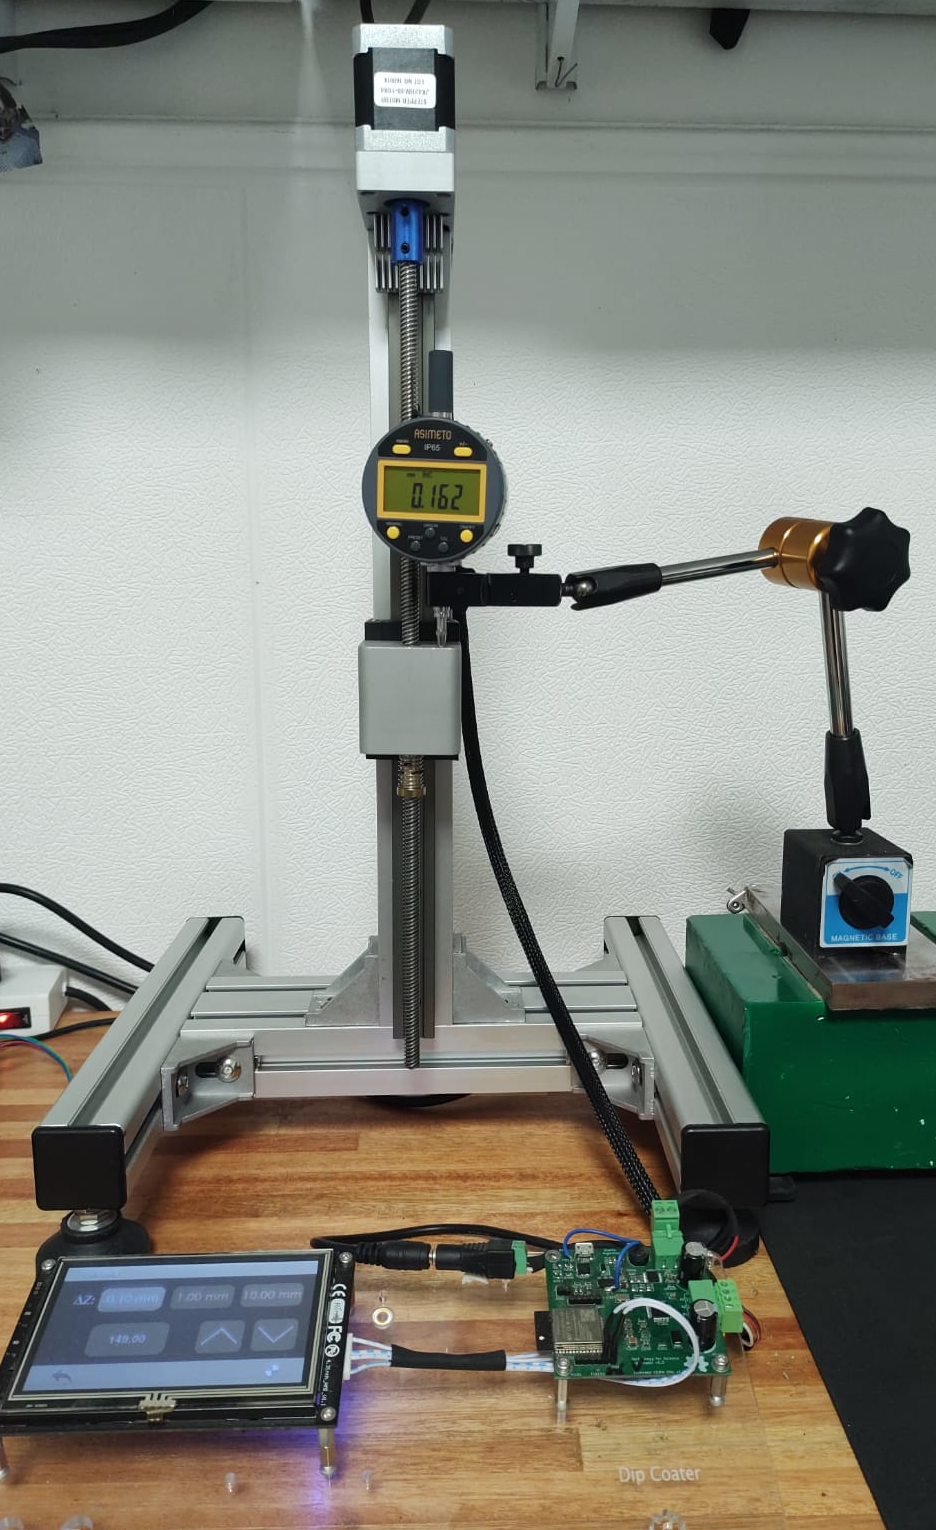
\includegraphics[width=.5\textwidth]{./Figures/desplazamiento_lineal.png}
	\caption{Ensayo de desplazamiento lineal con micrómetro.}
	\label{fig:desplazamiento_lineal}
\end{figure}

\begin{figure}[!ht]
	\centering
	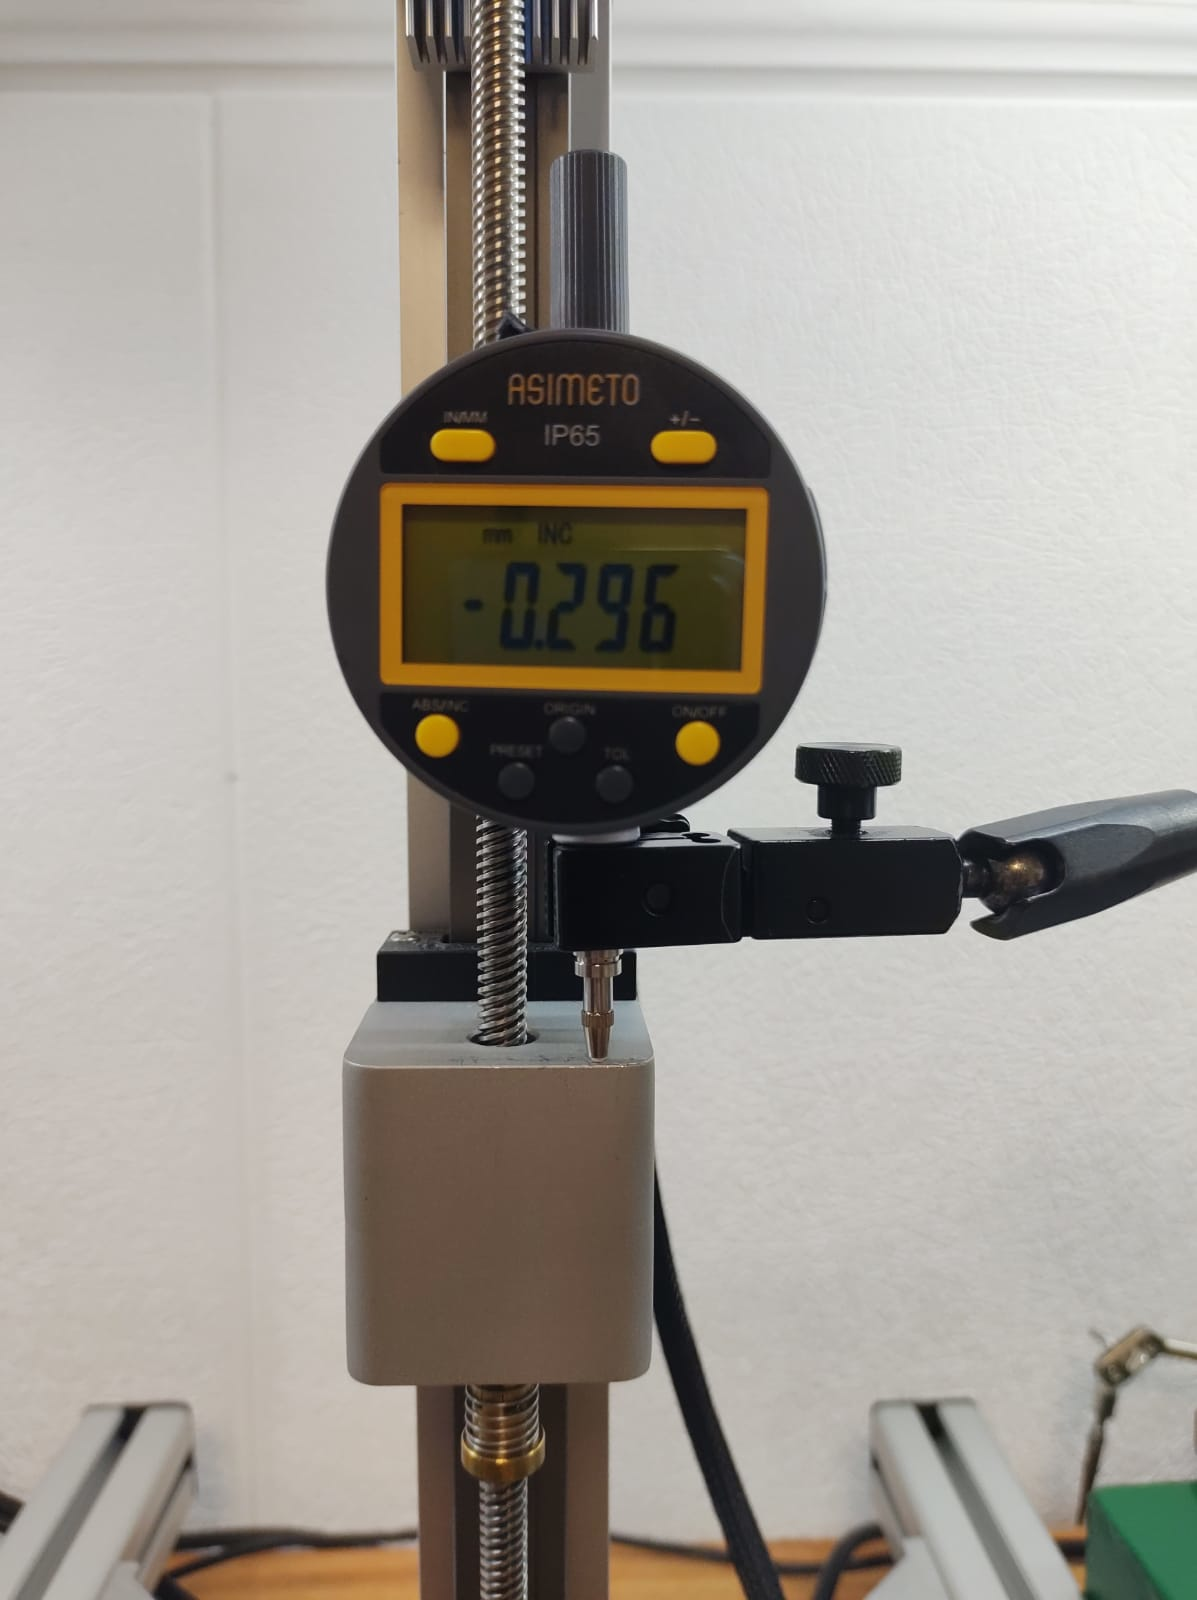
\includegraphics[width=.5\textwidth]{./Figures/micrometro.png}
	\caption{Micrómetro digital Asimeto.}
	\label{fig:micrometro}
\end{figure}


\section{Pruebas de campo con personal capacitado}